\documentclass[11pt]{article}
\usepackage{amsmath, amssymb, amsfonts}
\usepackage[margin=1in]{geometry}
\usepackage{fancyhdr}
\usepackage{tcolorbox}
\usepackage{enumerate}
\usepackage{tikz}
\usepackage{algorithmic}


\newcommand{\zo}{\{0,1\}}
\usetikzlibrary{shapes.geometric,arrows,fit,matrix,positioning}
\tikzset
{
    treenode/.style = {circle, draw=black, align=center, 
                          minimum size=1cm, anchor=center}
}

\begin{document}

    \setlength{\headheight}{26pt}
    \pagestyle{fancy}
    \fancyhead[C]{\textbf{Basic Algorithms (Section 5)}\\Spring 2025}
    \fancyhead[R]{HW7 (Due 4/3 23:59)\\ Instructor: Jiaxin Guan}
    \fancyfoot[C]{}
    \fancyfoot[R]{\thepage}
    \renewcommand{\headrulewidth}{0.4pt}
    \renewcommand{\footrulewidth}{0.4pt}
    
    %%%% EDIT THIS PART 
    %Put your name and Net ID here
	\fancyhead[L]{Name: Nick Zhu \\ Net ID: xz4687}
    %Write your collaborators' names here
    \fancyfoot[L]{Discussion Partners:}
    %%%%%

    %Problem 1
    \begin{tcolorbox}[title={Problem 1 (Interval Scheduling with Revenue, 35 pts)}] \setlength\parindent{1em}
        During the lecture we considered the activity selection/interval scheduling problem, where the goal is to schedule as many non-overlapping activities/intervals as possible. 
        
        Now suppose instead of maximizing the number of activities scheduled, we modify the problem by adding ``revenue'' value $r_i$ to each activity $I_i$, for all $i$. The modified goal is to find a set of non-overlapping activities $S'\subseteq S$ that maximizes the total revenue, defined as \[
        \sum_{I_i\in S'} r_i.\]

        \begin{enumerate}[(a)]
        \item Does the greedy algorithm presented in class correctly solve
        this problem? If yes, provide a brief justification. If no, provide a counterexample.
        \item What about the improved DP algorithm (the one with $O(n\log n)$ runtime) presented in class? Can it be easily adapted to solve this problem? If yes, briefly describe what changes need to be made. If no,  provide a brief justification.
        \end{enumerate}
            
    \end{tcolorbox}
    %Write your solution here!
    \section*{Solution}

    \subsection*{(a)}
    The greedy algorithm presented in class does not correctly solve this problem. 

    \medskip
    \noindent\textbf{Counterexample:} Consider the following intervals:
    \begin{itemize}
        \item \( I_1 \): starts at time 0, ends at time 2, with revenue \( r_1 = 1 \).
        \item \( I_2 \): starts at time 2, ends at time 4, with revenue \( r_2 = 1 \).
        \item \( I_3 \): starts at time 0, ends at time 4, with revenue \( r_3 = 3 \).
    \end{itemize}
    The greedy algorithm based on the earliest finish time would select \( I_1 \) and \( I_2 \), yielding a total revenue of \( 1 + 1 = 2.\)
    However, the optimal solution is to select \( I_3 \) alone, which gives a revenue of 3.
    
    \subsection*{(b)}
    Yes, the improved DP algorithm can be adapted to solve this problem.
    
    \medskip
    \noindent For this problem, we need to includethe revenue of each interval into the recurrence. After sorting the intervals by finish time, define:
    \[
    \text{DP}[j] = \max\{r_j + \text{DP}[p(j)],\, \text{DP}[j-1]\},
    \]
    \begin{itemize}
        \item \( r_j \) is the revenue of interval \( I_j \).
        \item \( p(j) \) is the index of the rightmost interval that finishes before \( I_j \) starts (i.e., the largest index \( i < j \) such that \( f_i \le s_j \)).
    \end{itemize}
    
    \medskip
    \noindent This rucurrence chooses between including interval \( I_j \) (and adding its revenue plus the best revenue from compatible intervals) or excluding \( I_j \) (and taking the best revenue from the previous intervals). 

    \noindent Since \( p(j) \) can be computed in \( O(\log n) \) time using binary search, the overall runtime remains \( O(n \log n) \).
    


    \newpage


    %Problem 2
    \begin{tcolorbox}[title={Problem 2 (Min Interval Scheduling, 35 pts)}] \setlength\parindent{1em}
        In the interval scheduling problem, we are given a set of intervals $S=\{[s_1, f_1],\dots,[s_n,f_n]\}$ and we want to find the largest subset $S'\subseteq S$ such that no two intervals in $S'$ overlap. 

        Now suppose that instead of wanting to prevent overlap, we want to prevent having any empty areas. That is, we want that for every point $p \in [a, b]$, there is some interval $I = [s,f] \in S'$ such that $s \leq p \leq f$. We say that such a set $S'$ \emph{covers} $[a,b]$.
        
        For example, on input $S = \{[0,5], [2,6], [3, 8], [7, 10], [9, 10]\}$, with target $[a,b] = [0, 10]$ an optimal covering is $S' = \{[0,5], [3,8], [7, 10]\}$.
        
        Given a set of $n$ intervals $S$ and a target interval $[a,b]$, we want to construct an efficient greedy algorithm to find the smallest $S' \subseteq S$ such that $S'$ covers $[a,b]$.
        
        \begin{enumerate}[(a)]
            \item Consider the greedy strategy where we always choose the interval $I$ which covers the largest amount of uncovered area of the target interval. Construct a counterexample such that this greedy strategy leads to a suboptimal solution.
            \item Give a greedy strategy that is safe. Prove that your greedy choice combined with an optimal solution to the subproblem remaining (after you make your greedy choice) is an optimal solution to the problem.
            \item Describe a full algorithm that implements your greedy strategy and analyze its running time. For full credit, your algorithm should run in time $O(n\log n)$.
        \end{enumerate}
    \end{tcolorbox}
    %Write your solution here!
    \section*{Solution}
    \noindent\textbf{(a)} 
    \medskip
    \noindent \textbf{Counterexample:} Let 
    \[
    [a,b] = [0,10]
    \]
    and let 
    \[
    S = \{\, I_1 = [0,2],\quad I_2 = [1,9],\quad I_3 = [2,10] \,\}.
    \]
    Initially, the uncovered portion is \([0,10]\). Suppose algorithm breaks ties arbitrarily and selects \(I_2 = [1,9]\) because it covers 8 units. Then the remaining uncovered portions are \([0,1]\) and \([9,10]\). To cover these gaps, the algorithm must select at least one interval for each gap. For instance, it might choose:
    \[
    I_1 \text{ to cover } [0,1] \quad \text{and} \quad I_3 \text{ to cover } [9,10].
    \]
    Thus, the algorithm returns the covering \(\{I_2, I_1, I_3\}\) with 3 intervals. However, observe that the set 
    \[
    \{I_1, I_3\}
    \]
    covers \([0,10]\) since \(I_1\) covers \([0,2]\) and \(I_3\) covers \([2,10]\). This is an optimal covering using only 2 intervals. Thus, the given greedy strategy is suboptimal.
    
    \bigskip
    \noindent\textbf{(b)}
    \medskip
    \begin{enumerate}
        \item Let \(x\) denote the leftmost point in \([a,b]\) that is not yet covered.
        \item Among all intervals \(I = [s,f]\) with \(s \le x\), choose the interval \(I^*\) that has the \emph{largest} finish time \(f\) (i.e., that extends farthest to the right).
        \item Add \(I^*\) to the solution and update \(x := f\).
    \end{enumerate}
    
    \medskip
    \noindent\textbf{Proof:} 
    
    Suppose there is an optimal solution \(S^*\) that covers \([a,b]\) and let \(I'\in S^*\) be the interval that covers the leftmost uncovered point \(x\). By our greedy rule, we chose an interval 
    \[
    I^* = [s^*,f^*] \quad \text{with } s^*\le x \quad \text{and} \quad f^* \ge f',
    \]
    where \(I' = [s',f']\). Replace \(I'\) with \(I^*\) in \(S^*\); the modified solution still covers \([a,b]\) and does not use more intervals. Then, the problem reduces to covering \([f^*,b]\). By applying the same argument recursively, we see that our greedy choice at each step leads to an overall optimal solution.
    
    \bigskip
    \noindent\textbf{(c)}
    
    \medskip
    \noindent\textbf{Algorithm:}
    \begin{enumerate}
        \item \textbf{Sort:} Sort the intervals in \(S\) by their starting times. (This takes \(O(n \log n)\) time.)
        \item \textbf{Initialize:} Set \(\text{current} \leftarrow a\) and \(S' \leftarrow \emptyset\).
        \item \textbf{While} \(\text{current} < b\):
        \begin{enumerate}
            \item Among all intervals \(I = [s,f]\) with \(s \le \text{current}\), choose the one with the maximum \(f\). (This can be done in a single pass using a pointer or by binary search as the intervals are sorted.)
            \item If no such interval exists, then there is no covering for \([a,b]\) and the algorithm terminates with failure.
            \item Add the chosen interval \(I^*\) to \(S'\) and update \(\text{current} \leftarrow f^*\).
        \end{enumerate}
        \item \textbf{Return} \(S'\).
    \end{enumerate}
    
    \medskip
    \noindent\textbf{Running Time Analysis:}
    
    \begin{itemize}
        \item Sorting the intervals takes \(O(n \log n)\).
        \item The while-loop makes one pass through the intervals. By using a pointer (or maintaining an index) to track the intervals with \(s \le \text{current}\), we can find the interval with the maximum \(f\) in \(O(1)\) time per interval (amortized). Hence, the loop runs in \(O(n)\) time.
    \end{itemize}
    
    Thus, the overall running time of the algorithm is \(O(n \log n)\).

    
    \newpage

    
    %Problem 3
    \begin{tcolorbox}[title={Problem 3 (Huffman Encoding Practice, 15 points)}] \setlength\parindent{1em}
        Consider a file that uses the symbols $\{A,B,C,D,E,F,G\}$ with the corresponding frequencies:
        
        \begin{center}
            \begin{tabular}{c|c|c|c|c|c|c}
               $f_A$  & $f_B$ & $f_C$ & $f_D$ & $f_E$ & $f_F$ & $f_G$ \\
               \hline
                0.08 & 0.12 & 0.14 & 0.15 & 0.28 & 0.13 & 0.1 \\
            \end{tabular}
        \end{center}

        Find an optimal prefix code based on Huffman’s algorithm (using $0$ and $1$ only). You should give out the following (no justification needed):
        
        \begin{enumerate}[(a)]
        \item The derived Huffman tree.
        \item The mapping from symbols to bit strings. (You can fill in the chart below)
        \begin{center}
            \begin{tabular}{c|c}
               Symbol & Encoding \\ 
               & (e.g. 1101)\\ \hline
                A & \\ \hline
                B & \\ \hline
                C & \\ \hline
                D & \\ \hline
                E & \\ \hline
                F & \\ \hline
                G & \\            
            \end{tabular}
        \end{center}
        \item $ABL$ (Average Bits per Letter) of your encoding.
        \end{enumerate}    
    \end{tcolorbox}
    %Write your solution here!
    \section*{Problem 3: Huffman Encoding Practice}

    Consider a file that uses the symbols $\{A,B,C,D,E,F,G\}$ with the corresponding frequencies:
    
    \begin{center}
    \begin{tabular}{c|c|c|c|c|c|c}
    $f_A$ & $f_B$ & $f_C$ & $f_D$ & $f_E$ & $f_F$ & $f_G$ \\ \hline
    0.08  & 0.12  & 0.14  & 0.15  & 0.28  & 0.13  & 0.10
    \end{tabular}
    \end{center}
    
    \vspace{0.2in}
    \textbf{(a) The Derived Huffman Tree:}
    
    The Huffman algorithm proceeds as follows:
    \begin{enumerate}
        \item \textbf{Initialization:} List the symbols with their frequencies:
        \[
        A(0.08),\quad G(0.10),\quad B(0.12),\quad F(0.13),\quad C(0.14),\quad D(0.15),\quad E(0.28).
        \]
        \item \textbf{Step 1:} Combine $A(0.08)$ and $G(0.10)$ to form a node with weight $0.18$.
        \item \textbf{Step 2:} Combine $B(0.12)$ and $F(0.13)$ to form a node with weight $0.25$.
        \item \textbf{Step 3:} Combine $C(0.14)$ and $D(0.15)$ to form a node with weight $0.29$.
        \item \textbf{Step 4:} Combine the nodes with weights $0.18$ and $0.25$ to form a node with weight $0.43$.
        \item \textbf{Step 5:} Combine $E(0.28)$ and the node with weight $0.29$ to form a node with weight $0.57$.
        \item \textbf{Step 6:} Finally, combine the nodes with weights $0.43$ and $0.57$ to form the root node with weight $1.0$.
    \end{enumerate}
    
    Below is a diagram of the Huffman tree using TikZ. In the tree, we assign a \textbf{0} to left branches and a \textbf{1} to right branches.
    
    \begin{center}
    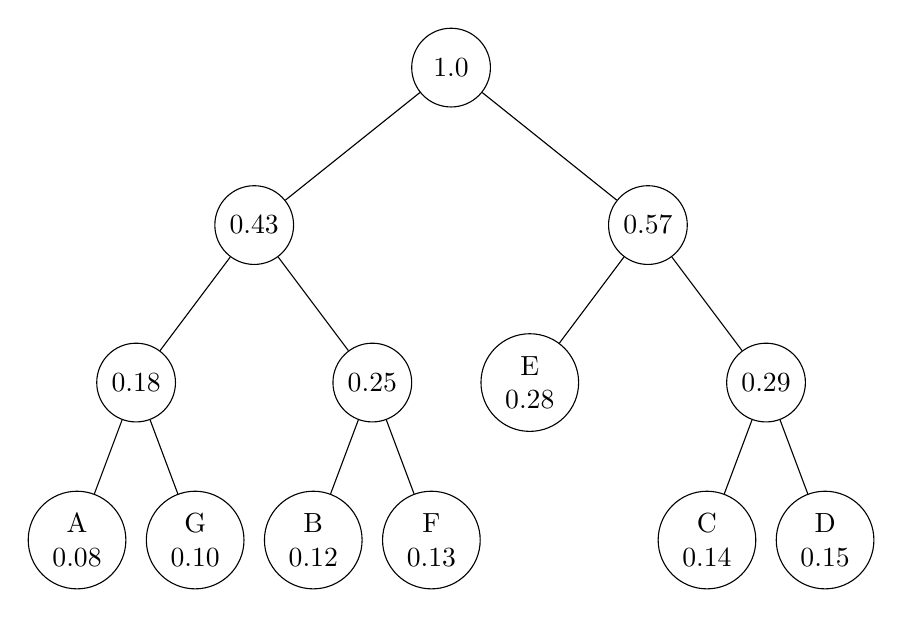
\begin{tikzpicture}[
        % Increase vertical distance between levels:
        level distance=2cm,
        % Set sibling distance for each level as desired:
        level 1/.style={sibling distance=5cm},
        level 2/.style={sibling distance=3cm},
        level 3/.style={sibling distance=1.5cm},
        every node/.style={treenode}
      ]
        \node {1.0}
            child { node {0.43}
                child { node {0.18}
                    child { node {A\\0.08} }
                    child { node {G\\0.10} }
                }
                child { node {0.25}
                    child { node {B\\0.12} }
                    child { node {F\\0.13} }
                }
            }
            child { node {0.57}
                child { node {E\\0.28} }
                child { node {0.29}
                    child { node {C\\0.14} }
                    child { node {D\\0.15} }
                }
            };
    \end{tikzpicture}
    \end{center}
    
    \bigskip
    \textbf{(b) Mapping from Symbols to Bit Strings:}
    
    Using the convention that left branches are labeled \textbf{0} and right branches \textbf{1}, we obtain the following encodings:
    \begin{center}
    \begin{tabular}{c|c}
    \textbf{Symbol} & \textbf{Encoding} \\ \hline
    A & 000 \\[0.2cm]
    G & 001 \\[0.2cm]
    B & 010 \\[0.2cm]
    F & 011 \\[0.2cm]
    E & 10  \\[0.2cm]
    C & 110 \\[0.2cm]
    D & 111 \\
    \end{tabular}
    \end{center}
    
    \bigskip
    \textbf{(c) Average Bits per Letter (ABL):}
    
    The average number of bits per letter is computed as:
    \[
    ABL = \sum_{x \in \{A,B,C,D,E,F,G\}} f_x \cdot \ell(x),
    \]
    where \(f_x\) is the frequency and \(\ell(x)\) is the length of the encoding for symbol \(x\).
    
    \[
    \begin{array}{rcl}
    \text{For } A: & 0.08 \times 3 &= 0.24, \\
    \text{For } G: & 0.10 \times 3 &= 0.30, \\
    \text{For } B: & 0.12 \times 3 &= 0.36, \\
    \text{For } F: & 0.13 \times 3 &= 0.39, \\
    \text{For } E: & 0.28 \times 2 &= 0.56, \\
    \text{For } C: & 0.14 \times 3 &= 0.42, \\
    \text{For } D: & 0.15 \times 3 &= 0.45. \\
    \end{array}
    \]
    
    Summing these contributions:
    \[
    ABL = 0.24 + 0.30 + 0.36 + 0.39 + 0.56 + 0.42 + 0.45 = 2.72.
    \]
    
    \bigskip
    \textbf{Final Answers:}
    \begin{itemize}
        \item \textbf{Huffman Tree:} See the diagram above.
        \item \textbf{Encoding:}
        \[
        \begin{array}{c|c}
        \text{Symbol} & \text{Encoding} \\ \hline
        A & 000 \\
        B & 010 \\
        C & 110 \\
        D & 111 \\
        E & 10 \\
        F & 011 \\
        G & 001 \\
        \end{array}
        \]
        \item \textbf{Average Bits per Letter:} \(2.72\).
    \end{itemize}
    \newpage

    % Problem 4
    \begin{tcolorbox}[title={Problem 4 (Huffman Encoding, Short Answers, 15 points)}] \setlength\parindent{1em}
        \begin{enumerate}[(a)]
        \item In general, for a given set of letters and corresponding frequencies, is Huffman encoding always ``length-unique''? That is, for any letter, will the length of its encoding always be the same across all valid Huffman trees constructed from the frequencies? Note that different letters may have the same frequency in the general case. If yes, justify in a few sentences. Otherwise, provide a counterexample.
        \item Is it possible that in an \emph{optimal} prefix code, a letter with a lower frequency has a shorter encoding than a
        letter with a higher frequency? If no, explain why not in a few sentences. Otherwise, provide an explicit example of the letter frequencies and the corresponding prefix code.
        \end{enumerate}    
    \end{tcolorbox}
    %Write your solution here!    
    
\end{document}